\documentclass[a4paper]{article}
\usepackage{titling}
\usepackage{authblk}
\usepackage{fancyhdr}
\usepackage{hyperref}
\usepackage{rsc}
\usepackage{siunitx}
\usepackage{graphicx}
\usepackage{mhchem}
\usepackage{amsmath}
\usepackage{listings}
\usepackage{color}

\definecolor{dkgreen}{rgb}{0,0.6,0}
\definecolor{gray}{rgb}{0.5,0.5,0.5}
\definecolor{mauve}{rgb}{0.58,0,0.82}

\lstset{frame=tb,
  language=Python,
  aboveskip=3mm,
  belowskip=3mm,
  showstringspaces=false,
  columns=flexible,
  basicstyle={\ttfamily},
  numbers=none,
  numberstyle=\tiny\color{gray},
  keywordstyle=\color{blue},
  commentstyle=\color{dkgreen},
  stringstyle=\color{mauve},
  breaklines=true,
  breakatwhitespace=true,
  tabsize=3
}
\DeclareSIUnit\Fahrenheit{\degree F}

\title{Lecture 3: Functions and modular code}
\author[1]{Dr Benjamin J. Morgan}
\author[1,2]{Dr Andrew R. McCluskey}
\affil[1]{Department of Chemistry, University of Bath, email: b.j.morgan@bath.ac.uk}
\affil[2]{Diamond Light Source, email: andrew.mccluskey@diamond.ac.uk}
\setcounter{Maxaffil}{0}
\renewcommand\Affilfont{\itshape\small}

\pagestyle{fancy}
\fancyhf{}
\rhead{CH40208}
\lhead{\thetitle}
\rfoot{\thepage}

\begin{document}
\maketitle

\section*{Aim}
This lecture will introduce how to simplify your code by writing functions and how to reuse code easily in many different places.

\section{Functions}

Occasionally, there is a particular section of your code that you would like to reuse over-and-over, without having to write the code over and over (as previously mentioned, programmers are lazy).
For this, we make use of \emph{functions}, the use of which will be familiar.
For example, we have used the \texttt{print()} function already in previous weeks, and the NumPy library contains a wide variety of functions, some of which were introduced last week.
However, this week we shall see how it is possible to write our own functions in Python.

The general syntax for \emph{defining} a function in Python is as follows,
\begin{lstlisting}
# Defining a function

def my_function(argument_1, argument_2):
    """
    Adds together two arguments.
    """
    result = argument_1 + argument_2
    return result
\end{lstlisting}
Above, we defined a function named \texttt{my\_function} which took two \emph{arguments}, added them together to produce a result, which was \emph{returned}.
Once defined it is possible to use this function in our code as follows,
\begin{lstlisting}
# Using our function

a = 1
b = 2
c = my_function(a, b)

print(c)
\end{lstlisting}
It can be seen when looking at the above example, that the object that is returned from the function is then assigned to the variable \texttt{c}.
The text immediately following the function definition line is the \emph{docstring}, this is important to help others understand the purpose of the function without having to read the code (basically it is a description of the function's action).

The above example of a function is relatively simple, just adding together two numbers.
However, a function can contain a large amount of code abstracted to a single line.
Furthermore, a well named function can increase the readibility of code significantly (consider the atomic distance code from previous weeks, the abstraction of the distance calculation to an appropriately named function would make this more understandable).

The \texttt{my\_function} example above contained two \emph{required} arguments.
These are the objects that are passed of the function when it is called (and typically these are operated on in some fashion) and are necessary for the function to run.
In addition to these required arguments, other arugments may be included in a given function; such as \emph{default} arguments and \emph{variable-length} arguments.
These are showing in the functions below,
\begin{lstlisting}
# A function with defaults

def my_function(arg1, arg2, arg3=0):
    """
    Adds together two arguments,
    and an optional third.
    """
    result = arg1 + arg2 + arg3
    return result

print(my_function(1, 2))
print(my_function(1, 2, arg3=3))

# A variable length argument

def my_function(arg1, arg2, *arg3):
    """
    Definitely adds together two arguments,
    but can optionally add together any
    number!
    """
    result = arg1 + arg2
    for i in arg3:
        result += i
    return result

print(my_function(1, 2))
print(my_function(1, 2, 3, 4, 5))
\end{lstlisting}
Note that in default argument example, if no value was given it would default to \texttt{0}.

You should be aware that a Python function does not \textbf{need} to have any arguments.
For example, you could write a function that returns the value of the Planck constant (ideally using the SciPy constants library),
\begin{lstlisting}
# A function with no arguments

from scipy import constants

def h():
    """
    Planck constant.
    """
    return constants.h

print('Planck constant = {:.3e}'.format(h()))
\end{lstlisting}

\vspace{\baselineskip}
\begin{center}
	\noindent\fbox{%
	    \begin{minipage}{0.9\textwidth}%
	        \vspace{0.15\baselineskip}
			\subsubsection*{Exercise}
        Investigate the effect of returning two values from a function, using the \texttt{return a, b} syntax.
	    \end{minipage}
	}
\end{center}

\section{Modules}

In addition to writing your own functions, it is possible to \emph{clean up} your code further by creating your own \emph{modules}.
These modules are similar to the libraries (like NumPy and SciPy) that we discussed last week, however, they are created by you.
This is achieved by creating a file in the folder where you would like to use the module, and then \emph{importing} the module in the code where your would like to use it.
For example, say you have a file called \texttt{atom\_helper.py} in which you will put many functions related to atomistic calculations.
Lets start it off with our distance calculation,
\begin{lstlisting}
# atom_helper.py

import numpy as np

def distance(a, b):
    """
    Determines the distance between two points
    in any number of dimensions.
    """
    return np.sqrt(np.sum(np.square(a - b)))
\end{lstlisting}
Having created this module, we can then import it into a Jupyter Notebook that is in the same folder, and access the distances function as shown below,
\begin{lstlisting}
# Using the atom_helper module

import numpy as np
import atom_helper

atom1 = np.array([1, 4, 2])
atom2 = np.array([5, 2, 6])

dist = atom_helper.distance(atom1, atom2)
print(dist)
\end{lstlisting}
It is clear from the above example, that the \emph{user-defined} module can be imported in the same way as a library.
Then any function defined in the module may be called from the Jupyter Notebook.
This means that you can create modules containing a wide variety of functions and use them in many different Notebooks.

\section{Problem 1: Energy minimisation}

It is possible to estimate the interaction energy, $E_{LJ}$ between two atoms using the Lennard-Jones expression,
\begin{equation}
  E_{LJ} = \frac{A}{r^{12}} - \frac{B}{r^6}
\end{equation}
where, $r$ is the distances between the two atoms, $A$ and $B$ are constants describing the shape of the interaction potential surface.
Add a function that can calculate the interaction energy, using the above relationship to the \texttt{atom\_helper.py} module; where the arguments are \texttt{r}, \texttt{A}, and \texttt{B}.

One of the most common operations in computational chemistry is energy minimisation, which is used to determine the most stable geometry for a given chemical molecule or structure.
The energy minimum is where there are no net forces acting on any of the atoms; the structure is relaxed.
This process will be covered in future lectures, however, in this exercise you will code the steps that can be found at the core of many energy-minimisation programs.

If $r_0$ is the initial distance between two atoms, and $E'$ and $E''$, respectively, are the first and second derivatives of the interaction energy, $E$, then a step towards the energy minimum is given by the following,
\begin{equation}
  r_1 = r_0 - \frac{E'}{E''},
\end{equation}
where, $r_1$ is the new distance between the two atoms.
We can then reevaluated $E'$ and $E''$ for the new $r$, and this process is repeated until $E$ reaches some minimum value.

For the purpose of this exercise, the interatomic interaction energy, $E$, and its derivatives are given by the followign reformulation of the Lennard-Jones equation,
\begin{equation}
  \begin{aligned}
    E & = \frac{A}{r^{12}} - \frac{B}{r^6} \\
    E' & = -12\frac{A}{r^{13}} + 6\frac{B}{r^7} \\
    E'' & = 156\frac{A}{r^{14}} - 42\frac{B}{r^8} \\
  \end{aligned}
\end{equation}

Write a program that, from values of $A$, $B$ and an initial guess of $r$, uses a 10 iteration loop to move towards the distance at which the energy minimum is present.
In each iteration: print a line containing the initial value of $r$ (i.e. $r_0$), $E$, $E'$, $E''$, and the final $r$ (i.e. $r_1$), and replace $r_0$ with $r_1$.
You will need to have three functions (one for each of $E$, $E'$, and $E''$) which will take $A$, $B$, and $r$ as their arguments.
\emph{Remember to plan the algorithm first!}

Given the following values for $A$ and $B$, what is the energy-minimum distance $r$ (in \AA)?
\begin{enumerate}
  \item{$A = \SI{1e5}{\eV\angstrom^{12}}$ and $B = \SI{40}{\eV\angstrom^{6}}$}
  \item{$A = \SI{4e5}{\eV\angstrom^{12}}$ and $B = \SI{1}{\eV\angstrom^{6}}$}
\end{enumerate}
Adjust the program so that it will do as many iterations as are necessary to achieve energy minimisation, rather than only a fixed number.
Compare cases 1. and 2. to see how stable and/or quick the minimisation is and how the \emph{convergence} depends on the initial guess of $r$.

\textbf{Extension}: Next, create a new function in your module to calculate the energy, and first and second derivatives of a harmonic oscillator (a common model for a covalent bond),
\begin{equation}
  \begin{aligned}
    E & = \frac{1}{2}k(r-r_{\text{eq}})^2 \\
    E' & = k(r-r_{\text{eq}}) \\
    E'' & = k \\
  \end{aligned}
\end{equation}
Verify that the method developed above (known as the Newton-Raphson method) converges to the energy minimum in a single step, regardless of the initial value of $r$, within this harmonic potential.
For this test, use $k = \SI{32.2}{\eV\angstrom^{-2}}$, which is the force constant for a \ce{HCl} molecule, and $r_{\text{eq}}=\SI{1.27}{\angstrom}$, where $r_{\text{eq}}$ is the equilibrium bond distance.

\section{Minimisation}

You might notice that if you start with a value for $r = 5$, then your energy minimisation will fail, going to larger and larger values of separation.
This is a problem with the Newton-Raphson minimisation algorithm that you have used; which assumes that the function being minimised is locally harmonic, and therefore the curvature will be positive.

One of the substantial benefits available from using the Python programming language is that for many problems there are already functions in publically available libraries that may be applied to our problems.
So instead of writting a custom, often very complex, minimisation algorithm it is easier to take advantage of the \texttt{scipy.optimize.minimize} function.
This can implement extremely powering local minimisation algorithms,
\begin{lstlisting}
# Easy optmisation

import numpy as np

def energy(r, A, B):
    """
    The Lennard-Jones potential
    """
    return A / np.power(r, 12) - B / np.power(r, 6)

from scipy.optimize import minimize

initial_guess = 4

results = minimize(energy, initial_guess, args=(1e5, 40))

print(results)
\end{lstlisting}
Note, that the first argument in the energy function is the value to be minimised, and the others have their values passed as default arguments to the \texttt{minimize} function using the \texttt{args} keyword.
\vspace{\baselineskip}
\begin{center}
	\noindent\fbox{%
	    \begin{minipage}{0.9\textwidth}%
	        \vspace{0.15\baselineskip}
			\subsubsection*{Exercise}
        Check that the \texttt{scipy.optimize.minimize} function is more stable to values of $r$ greater than 5.
        \textbf{Note}: That at values very far from the minimum, even the \texttt{scipy.optimize.minimize} function will struggle to reach a reasonable value.
	    \end{minipage}
	}
\end{center}

\section{Global optimisation}
%
\begin{figure}[t]
\centering
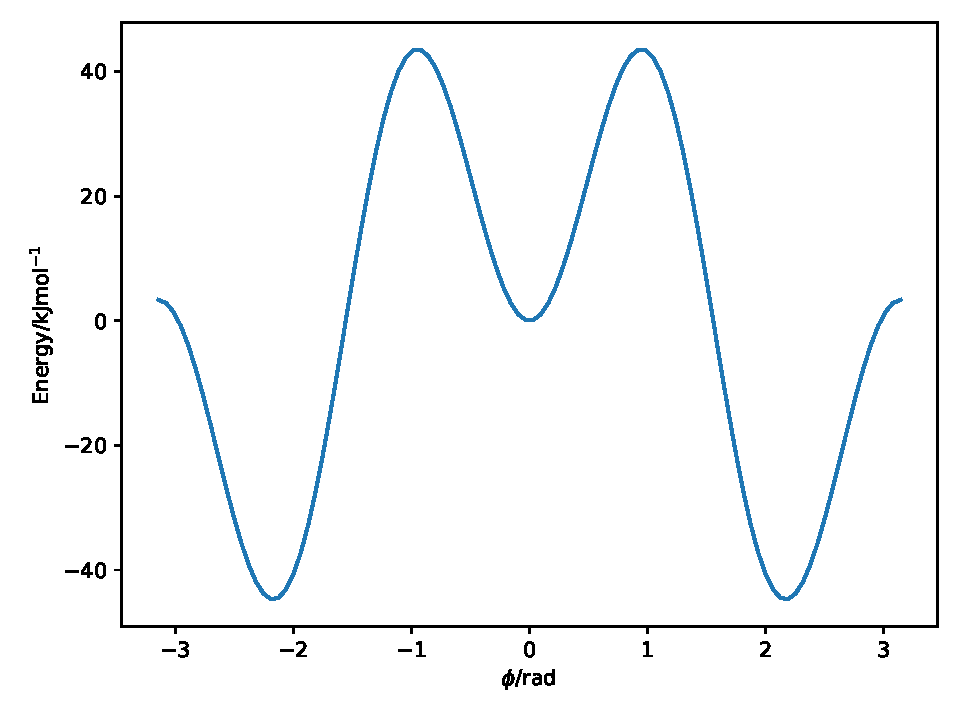
\includegraphics[width=0.6\textwidth]{dihedral}
\caption{\label{fig:dihed} The shape of the energy for a \ce{Cl-C-C-Cl} dihedral angle in 1,2-dichloroethane.}
\end{figure}
%

The energy of a \ce{Cl-C-C-Cl} dihedral angle in 1,2-dichloroethane may be described with the following function,
%
\begin{equation}
  E_{\text{dihedral}} = \frac{1}{2} \{A_1[1 + \cos(\phi)] + A_2[1 + \cos(2\phi)] + A_3[1 + \cos(3\phi)]\},
  \label{equ:dihed}
\end{equation}
%
where, $A_1 = \SI{55.229}{\kilo\joule\per\mole}$, $A_2 = \SI{3.3472}{\kilo\joule\per\mole}$, $A_3 = \SI{-58.576}{\kilo\joule\per\mole}$ and $\phi$ is the dihedral angle.

This is plotted from $-\pi$ to $\pi$ in Figure~\ref{fig:dihed}.
If you were to attempt to minimise the energy of this function, the initila starting position would be massively important on the resulting minimised value.
This is because the \texttt{scipy.optimize.minimize} function performs a local optimisation which means that typically it is not possible to the energy to increase and therefore can get stuck in small energy wells instead of finding the global solution.

Global minimisation is a large and active area of research in mathematics and computer science, as it is not easy to find a global solution for a function that may have many minima.
However, it is important to be aware that it is very easy for a minimisation (which are very common in computational chemistry) to get stuck in a local minimum and therefore be unable to probe the global minimum. 

%\bibliographystyle{rsc}
%\bibliography{handout_3}

\end{document}
